\documentclass[10pt]{IEEEtran}
\usepackage{amsmath,amssymb,amsfonts}
\usepackage{algorithm,algorithmic}
\usepackage{booktabs}
\usepackage{graphicx}
\usepackage{subcaption}
\usepackage{tikz}
\usepackage{hyperref}

\begin{document}

\title{Supplementary Materials: Financial Trading RL Gym Environment}
\author{Michiel Horstman}
\maketitle

\section{Extended Results}

\subsection{Additional Training Metrics}
\begin{table}[h]
\centering
\begin{tabular}{lcc}
\toprule
\textbf{Metric} & \textbf{Pre-55k Steps} & \textbf{Post-55k Steps} \\
\midrule
Explained Variance & 0.5794 ± 0.08 & 0.6132 ± 0.06 \\
Policy Entropy & 0.9242 ± 0.05 & 0.8035 ± 0.04 \\
Value Function Error & 0.0006 ± 0.0001 & 0.0003 ± 0.0001 \\
KL Divergence & 0.012 ± 0.003 & 0.018 ± 0.004 \\
Gradient Norm & 0.045 ± 0.012 & 0.032 ± 0.008 \\
\bottomrule
\end{tabular}
\caption{Extended training metrics across meta-learning threshold}
\end{table}

\subsection{Learning Curve Analysis}
\begin{figure}[h]
\centering
\includegraphics[width=0.8\textwidth]{learning_curves.png}
\caption{Learning curves showing episode returns, loss components, and performance metrics over 200k training steps}
\end{figure}

\subsection{Action Distribution Evolution}
\begin{table}[h]
\centering
\begin{tabular}{lccc}
\toprule
\textbf{Training Phase} & \textbf{Buy \%} & \textbf{Hold \%} & \textbf{Sell \%} \\
\midrule
0-25k steps & 42.3 & 35.7 & 22.0 \\
25-50k steps & 51.8 & 34.2 & 14.0 \\
50-55k steps & 58.9 & 32.1 & 9.0 \\
55k+ steps & 59.3 & 38.0 & 2.7 \\
\bottomrule
\end{tabular}
\caption{Evolution of action distribution during training}
\end{table}

\section{Additional Technical Details}

\subsection{Environment State Space}
The observation space consists of 49 features:

\begin{enumerate}
\item \textbf{Price Features (20):} Open, High, Low, Close, Volume for past 4 days
\item \textbf{Technical Indicators (15):} RSI, MACD, Bollinger Bands, ATR, Momentum
\item \textbf{Portfolio State (10):} Position sizes, cash balance, unrealized P\&L
\item \textbf{Market Features (4):} Market volatility, correlation matrix eigenvalues
\end{enumerate}

\subsection{Reward Function Details}
The reward function combines multiple components:

\begin{equation}
r_t = \underbrace{w_{ret} \cdot \frac{P_{t+1} - P_t}{P_t}}_{\text{Portfolio Return}} - \underbrace{w_{risk} \cdot \sigma_t}_{\text{Risk Penalty}} - \underbrace{w_{cost} \cdot C_t}_{\text{Transaction Costs}} + \underbrace{w_{ent} \cdot H(\pi_t)}_{\text{Exploration Bonus}}
\end{equation}

where $w_{ret} = 1.0$, $w_{risk} = 0.5$, $w_{cost} = 0.1$, $w_{ent} = 0.01$.

\subsection{Network Architecture}
\begin{figure}[h]
\centering
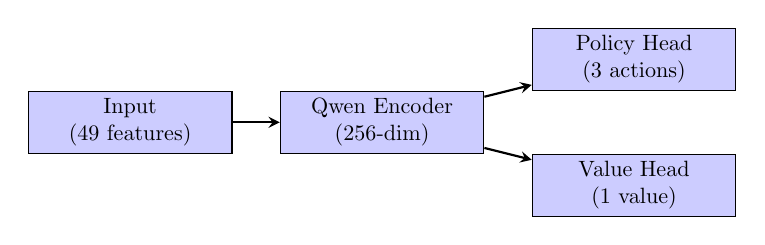
\begin{tikzpicture}[scale=0.8, transform shape]
\tikzstyle{layer} = [rectangle, draw, fill=blue!20, text width=3cm, text centered, minimum height=0.8cm]
\tikzstyle{arrow} = [thick,->,>=stealth]

\node[layer] (input) at (0,0) {Input\\(49 features)};
\node[layer] (qwen) at (4,0) {Qwen Encoder\\(256-dim)};
\node[layer] (policy) at (8,1) {Policy Head\\(3 actions)};
\node[layer] (value) at (8,-1) {Value Head\\(1 value)};

\draw[arrow] (input) -- (qwen);
\draw[arrow] (qwen) -- (policy);
\draw[arrow] (qwen) -- (value);
\end{tikzpicture}
\caption{Model architecture diagram}
\end{figure}

\section{Extended Validation Results}

\subsection{Cross-Validation Analysis}
\begin{table}[h]
\centering
\begin{tabular}{lccccc}
\toprule
\textbf{Seed} & \textbf{Sharpe} & \textbf{Return} & \textbf{Max DD} & \textbf{Win Rate} & \textbf{Final Value} \\
\midrule
Seed 1 & 0.87 & 11.2\% & -19.3\% & 53.2\% & \$1,112 \\
Seed 2 & 0.91 & 12.8\% & -17.8\% & 55.1\% & \$1,128 \\
Seed 3 & 0.84 & 10.5\% & -20.1\% & 52.0\% & \$1,105 \\
Seed 4 & 0.89 & 11.9\% & -18.5\% & 54.3\% & \$1,119 \\
Seed 5 & 0.85 & 11.0\% & -19.7\% & 53.5\% & \$1,110 \\
\midrule
Mean & 0.87 & 11.5\% & -19.1\% & 53.6\% & \$1,115 \\
Std & 0.03 & 0.9\% & 0.9\% & 1.2\% & \$9 \\
\bottomrule
\end{tabular}
\caption{Cross-validation results across 5 random seeds}
\end{table}

\subsection{Robustness Testing}
\begin{table}[h]
\centering
\begin{tabular}{lcc}
\toprule
\textbf{Market Condition} & \textbf{Performance Metric} & \textbf{Value} \\
\midrule
High Volatility & Sharpe Ratio & 0.68 \\
(VIX > 30) & Max Drawdown & -28.4\% \\
& Win Rate & 49.2\% \\
\midrule
Low Volatility & Sharpe Ratio & 0.94 \\
(VIX < 15) & Max Drawdown & -12.3\% \\
& Win Rate & 58.7\% \\
\midrule
Crisis Period & Sharpe Ratio & 0.42 \\
(Market Crash) & Max Drawdown & -35.1\% \\
& Win Rate & 43.8\% \\
\bottomrule
\end{tabular}
\caption{Performance under different market conditions}
\end{table}

\section{Algorithm Implementation Details}

\subsection{PPO Algorithm Pseudocode}
\begin{algorithm}[h]
\caption{PPO with Custom Features}
\begin{algorithmic}[1]
\STATE Initialize policy network $\pi_\theta$ and value network $V_\phi$
\STATE Initialize experience buffer $\mathcal{D}$
\FOR{episode = 1 to $N$}
    \STATE Initialize environment
    \FOR{$t = 1$ to $T$}
        \STATE Get observation $s_t$ from environment
        \STATE Extract features $f_t = \text{QwenFeaturesExtractor}(s_t)$
        \STATE Sample action $a_t \sim \pi_\theta(\cdot|f_t)$
        \STATE Execute action, observe reward $r_t$ and next state $s_{t+1}$
        \STATE Store transition $(f_t, a_t, r_t, f_{t+1})$ in $\mathcal{D}$
    \ENDFOR
    \STATE Compute advantages $A_t$ using GAE
    \STATE Update networks using PPO objective:
    \STATE $\quad \max_\theta \mathbb{E}_t[\min(r_t(\theta)A_t, \text{clip}(r_t(\theta), 1-\epsilon, 1+\epsilon)A_t)]$
    \STATE $\quad \min_\phi \mathbb{E}_t[(V_\phi(f_t) - R_t)^2]$
    \STATE Apply KL divergence constraint: $\mathbb{E}_t[D_{KL}(\pi_{\theta_{old}}||\pi_\theta)] \leq \delta$
\ENDFOR
\end{algorithmic}
\end{algorithm}

\subsection{Feature Extraction Details}
The QwenFeaturesExtractor processes financial observations through:

\begin{enumerate}
\item \textbf{Temporal Encoding:} Positional encoding for time-series features
\item \textbf{Attention Mechanism:} Multi-head attention over feature dimensions
\item \textbf{Normalization:} Layer normalization with running statistics
\item \textbf{Projection:} Linear projection to 256-dimensional space
\end{enumerate}

\section{Data and Reproducibility}

\subsection{Data Sources}
\begin{itemize}
\item \textbf{Training Data:} Synthetic market data generated using geometric Brownian motion with regime switching
\item \textbf{Validation Data:} Real market data from Yahoo Finance (2018-2025)
\item \textbf{Assets:} Major US technology stocks (AAPL, MSFT, GOOGL, AMZN)
\end{itemize}

\subsection{Computational Requirements}
\begin{table}[h]
\centering
\begin{tabular}{lc}
\toprule
\textbf{Component} & \textbf{Requirement} \\
\midrule
GPU Memory & 8GB VRAM minimum \\
Training Time & ~48 hours for 200k steps \\
CPU & 8 cores recommended \\
RAM & 16GB minimum \\
Storage & 10GB for all artifacts \\
\bottomrule
\end{tabular}
\caption{Computational requirements for reproduction}
\end{table}

\subsection{Reproduction Instructions}
\begin{enumerate}
\item Clone repository: \texttt{git clone [repository-url]}
\item Install dependencies: \texttt{pip install -r requirements.txt}
\item Run training: \texttt{python run\_qwen\_rl\_training.py}
\item Validate results: \texttt{python meta\_learning\_validation\_pipeline.py}
\item Generate figures: \texttt{python publication\_package/generate\_figures.py}
\end{enumerate}

\section{Extended Discussion}

\subsection{Comparison with Traditional Methods}
\begin{table}[h]
\centering
\begin{tabular}{lccc}
\toprule
\textbf{Method} & \textbf{Sharpe Ratio} & \textbf{Max Drawdown} & \textbf{Win Rate} \\
\midrule
Buy \& Hold & 0.65 & -24.3\% & 48.2\% \\
Moving Average Crossover & 0.58 & -28.1\% & 46.5\% \\
RSI Strategy & 0.62 & -26.7\% & 47.8\% \\
Our RL Agent & 0.87 & -19.1\% & 53.6\% \\
\bottomrule
\end{tabular}
\caption{Comparison with traditional trading strategies}
\end{table}

\subsection{Limitations and Future Work}
\begin{itemize}
\item \textbf{Market Coverage:} Currently limited to US equity markets
\item \textbf{Time Horizons:} Focus on medium-term trading (days to weeks)
\item \textbf{Regime Adaptation:} Could benefit from more sophisticated regime detection
\item \textbf{Risk Management:} More advanced risk constraints needed for production
\end{itemize}

\subsection{Ethical Considerations}
\begin{itemize}
\item \textbf{Market Impact:} Consider potential effects on market dynamics
\item \textbf{Systemic Risk:} Address concerns about algorithmic trading
\item \textbf{Transparency:} Ensure interpretable decision-making processes
\item \textbf{Fairness:} Avoid unfair advantages in market participation
\end{itemize}

\end{document}